\documentclass{beamer}

\usetheme{Darmstadt}
\usepackage{graphics}
\usepackage{caption}
\usepackage{hyperref}

\title{Benzene, Limma, LASSO, Super Learner -- what more could you want on a Thursday afternoon?}
\subtitle{make sure you're sitting down for this...}
\author{Courtney Schiffman, Partow Imani, Rebecca Hyde, Nima Hejazi}
\institute[UC Berkeley]{University of California, Berkeley}
\date{December 10, 2015}

\setbeamercovered{transparent}
\setbeamertemplate{navigation symbols}{}

\begin{document}

\frame{\titlepage}

\section[Outline]{}
\frame{\tableofcontents}


\section{Introduction}

\begin{frame}
	\frametitle{Contents}
	\tableofcontents[currentsection,currentsubsection,hideothersubsections,sectionstyle=show/shaded] 
\end{frame}


\subsection{Background}

\begin{frame}[fragile]
  	\frametitle{Benzene, Genes, and Health}
	\begin{itemize}
  			\item Data was collected on 77 subjects -- with some exposed to benzene, and others as control.
			\item Gene expression patterns were measured using a new sequencing technology -- \textit{nCounter.}
 			\item Super Learner was used to ascertain the minimum number of genes necessary to predict benzene exposure with relative accuracy.
  			\item Found 6 genes (PRG2, AQP9, NFKB1, ACSL1, CLEC5A, IFNB1) with good prediction accuracy.
  		\end{itemize}
\end{frame}

\subsection{Overview}

\begin{frame}[fragile]
  	\frametitle{A Roadmap of Our Analysis}
 		\begin{itemize}
  			\item Limma was used to find differential expression measures for all exposures in the PBMC data sets.
			\item Super Learner was used (with a small library), and \textit{cvAUC} was used to evaluate the performance of our predictors of interest (gene pairs).
			\item LASSO regression was used to compare the performance of a simpler (parametric) method with that of Super Learner.
  		\end{itemize}
\end{frame}

\section{Methodology}

\begin{frame}
        \frametitle{Contents}
        \tableofcontents[currentsection,currentsubsection,hideothersubsections,sectionstyle=show/shaded]
\end{frame}

\subsection{Differential Gene Expression}

\begin{frame}[fragile]
	\frametitle{\textit{Limma} for Gene Expression Analysis}
 		\begin{itemize}
			\item \textit{Limma} --- Linear Models for Microarray Data (Bioconductor R package).
			\item Linear models were used to predict gene expression based on treatment and control status.
			\item An empirical Bayes method was used to create a moderated t-statistic for each contrast coefficient.
			\item The false discovery rate was controlled by adjusting for multiple testing via the Benjamini-Hochberg procedure.
		\end{itemize}
\end{frame}

\subsection{The Super Learner Algorithm}

\begin{frame}
	\frametitle{How Does Super Learner Work?}
		\begin{center}
    			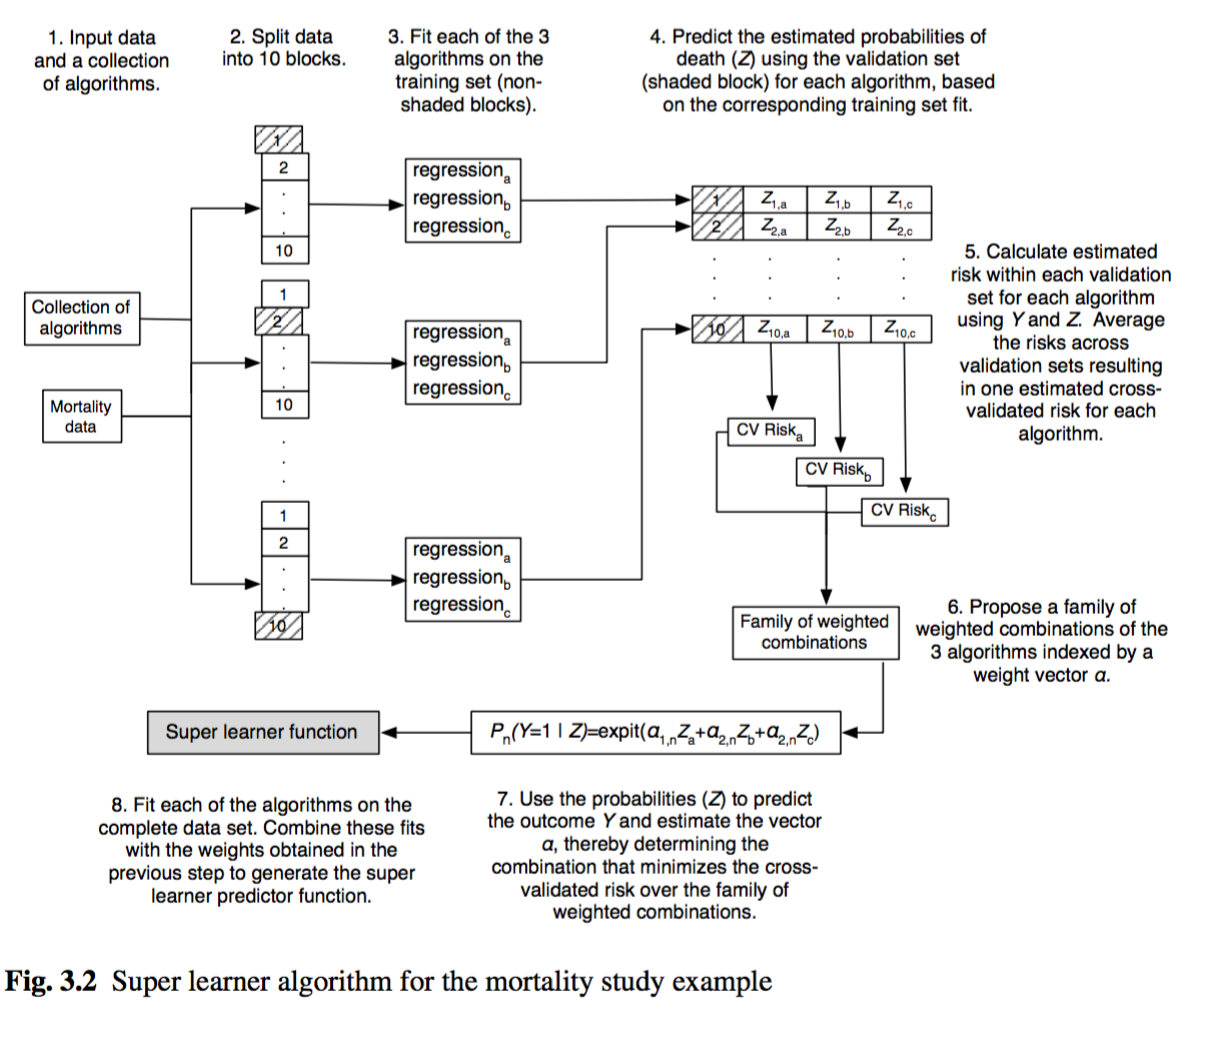
\includegraphics[scale=0.45]{../paper/figs/SuperLearn2.png}
		\end{center}
\end{frame}

\subsection{Cross-Validated AUC}

\begin{frame}[fragile]
  	\frametitle{cvAUC -- efficient AUC estimation for ROC curves}
 		$$AUC(P_{0},\psi) = \int_{0}^{1} P_{0}(\psi(X) > c | Y=1) P_{0}(\psi(X) = c | Y=0) dc$$
		\begin{itemize}
			\item This package reports cross-validated AUC and computes confidence intervals for cross-validated AUC estimates based on influence curves. This is computationally efficient (and feasible whereas use of the bootstrap is intractable in cases with large data sets).
			\item \textit{cvAUC} was used here to compute AUC estimates for ROC curves of the prediction of exposures in the PBMC data sets using specific pairs of genes.
		\end{itemize}
\end{frame}

\subsection{LASSO Regression}

\begin{frame}[fragile]
  	\frametitle{LASSO for Pairwise Gene Selection, part I}
		\centering
 		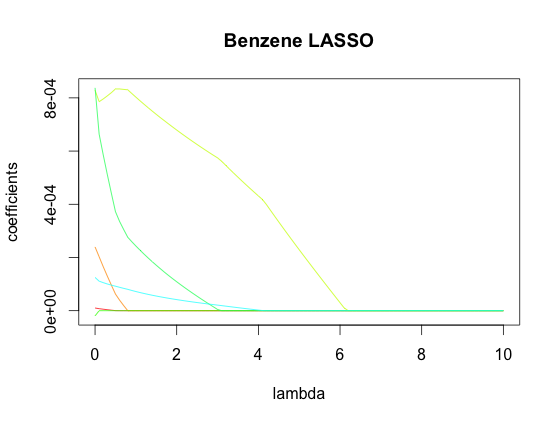
\includegraphics[scale=0.5]{../paper/figs/lasso_coef.png}
\end{frame}

\begin{frame}[fragile]
        \frametitle{LASSO for Pairwise Gene Selection, part II}
		\centering
                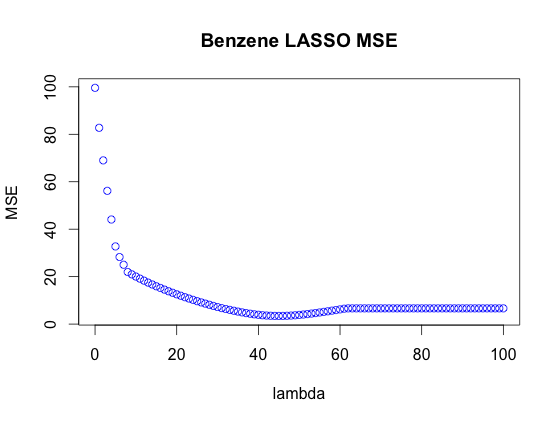
\includegraphics[scale=0.5]{../paper/figs/lasso_mse.png} 
\end{frame}

\section{Results}

\begin{frame}
        \frametitle{Contents}
        \tableofcontents[currentsection,currentsubsection,hideothersubsections,sectionstyle=show/shaded]
\end{frame}

\subsection{Differential Expression in Exposures}

\begin{frame}[fragile]
  	\frametitle{Differential Expression --- Benzene}
 		\begin{table}[ht]
		\caption {Differential expression in benzene exposure} \label{tab:benzene} 
		\centering
		\begin{tabular}{rlrrr}
  			\hline
 			Gene & Ratio & P-value & Q-value \\ 
  			\hline
			ACSL1 & 1.86 & 0.00 & 0.00 \\ 
  			AQP9 & 2.44 & 0.00 & 0.00 \\ 
  			CLEC5A & 2.39 & 0.00 & 0.00 \\ 
  			IFNB1 & 3.06 & 0.00 & 0.00 \\ 
  			NFKB1 & 1.64 & 0.00 & 0.00 \\ 
  			PRG2 & 1.67 & 0.01 & 0.02 \\ 
   			\hline
		\end{tabular}
		\end{table}
		\small Ratio is the $log_{2}$ fold change in expression values between the treatment and control. 
\end{frame}

\begin{frame}
	\frametitle{Benzene ROC curve (AQP9 \& ACSL1)}
		\centering
	 	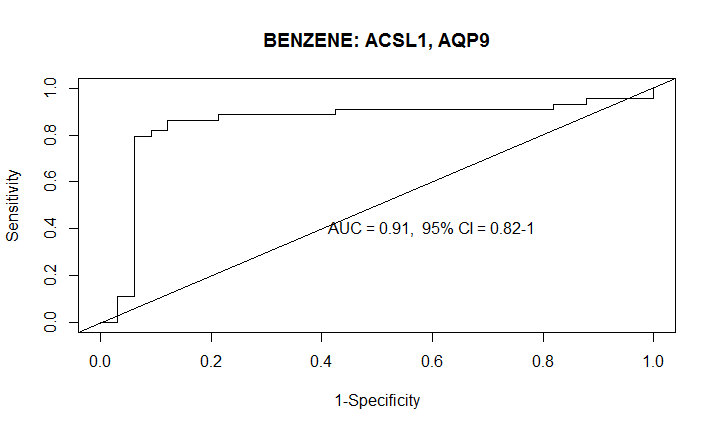
\includegraphics[scale=0.45]{../paper/figs/benzene1.png} 
\end{frame}

\begin{frame}[fragile]
  	\frametitle{Differential Expression --- Nickel}
 		\begin{table}[ht]
		\caption {Differential expression in nickel exposure} \label{tab:nickel} 
		\centering
		\begin{tabular}{rrrrrr}
 			\hline
 			& logFC & AveExpr & t & P.Value & adj.P.Val \\ 
  			\hline
			NFKB1 & 1.11 & 9.65 & 5.63 & 0.00 & 0.00 \\ 
  			ACSL1 & 0.88 & 9.47 & 4.92 & 0.00 & 0.00 \\ 
  			PRG2 & -0.48 & 5.32 & -4.42 & 0.00 & 0.00 \\ 
  			IFNB1 & -0.41 & 3.83 & -3.93 & 0.00 & 0.00 \\ 
  			AQP9 & 1.02 & 9.53 & 3.70 & 0.00 & 0.00 \\ 
  			CLEC5A & -0.11 & 5.88 & -0.85 & 0.40 & 0.47 \\ 
  			 \hline
		\end{tabular}
		\end{table}
		\small logFC is the $log_{2}$ fold change in expression values between the treatment and control.
\end{frame}

\begin{frame}
	\frametitle{Nickel ROC curve (AQP9 \& ACSL1)}
		\centering
	 	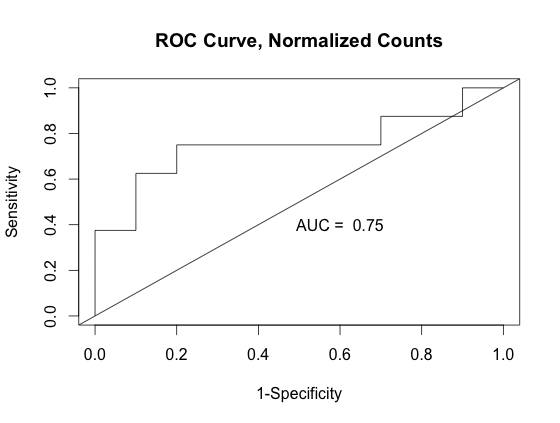
\includegraphics[scale=0.45]{../paper/figs/Nickel_ASCL1-APQ9.png} 
\end{frame}


\begin{frame}[fragile]
  	\frametitle{Differential Expression --- Smoking}
 		\begin{table}[ht]
		\caption {Differential expression in smoking exposure} \label{tab:smoking} 
		\centering
		\begin{tabular}{rrrrrr}
 		 	\hline
 			& logFC & AveExpr & t & P.Value & adj.P.Val \\ 
 			 \hline
			PRG2 & 0.12 & 4.49 & 1.04 & 0.31 & 1.00 \\ 
  			AQP9 & 0.18 & 7.56 & 0.62 & 0.54 & 1.00 \\ 
  			NFKB1 & 0.14 & 8.01 & 0.61 & 0.54 & 1.00 \\ 
  			ACSL1 & -0.27 & 6.71 & -0.58 & 0.56 & 1.00 \\ 
  			CLEC5A & -0.12 & 4.43 & -0.52 & 0.61 & 1.00 \\ 
  			IFNB1 & -0.02 & 4.49 & -0.13 & 0.90 & 1.00 \\ 
  			\hline
		\end{tabular}
		\end{table}
		\small logFC is the $log_{2}$ fold change in expression values between the treatment and control.
\end{frame}

\begin{frame}
	\frametitle{Smoking ROC curve (AQP9 \& ACSL1)}
		\centering
	 	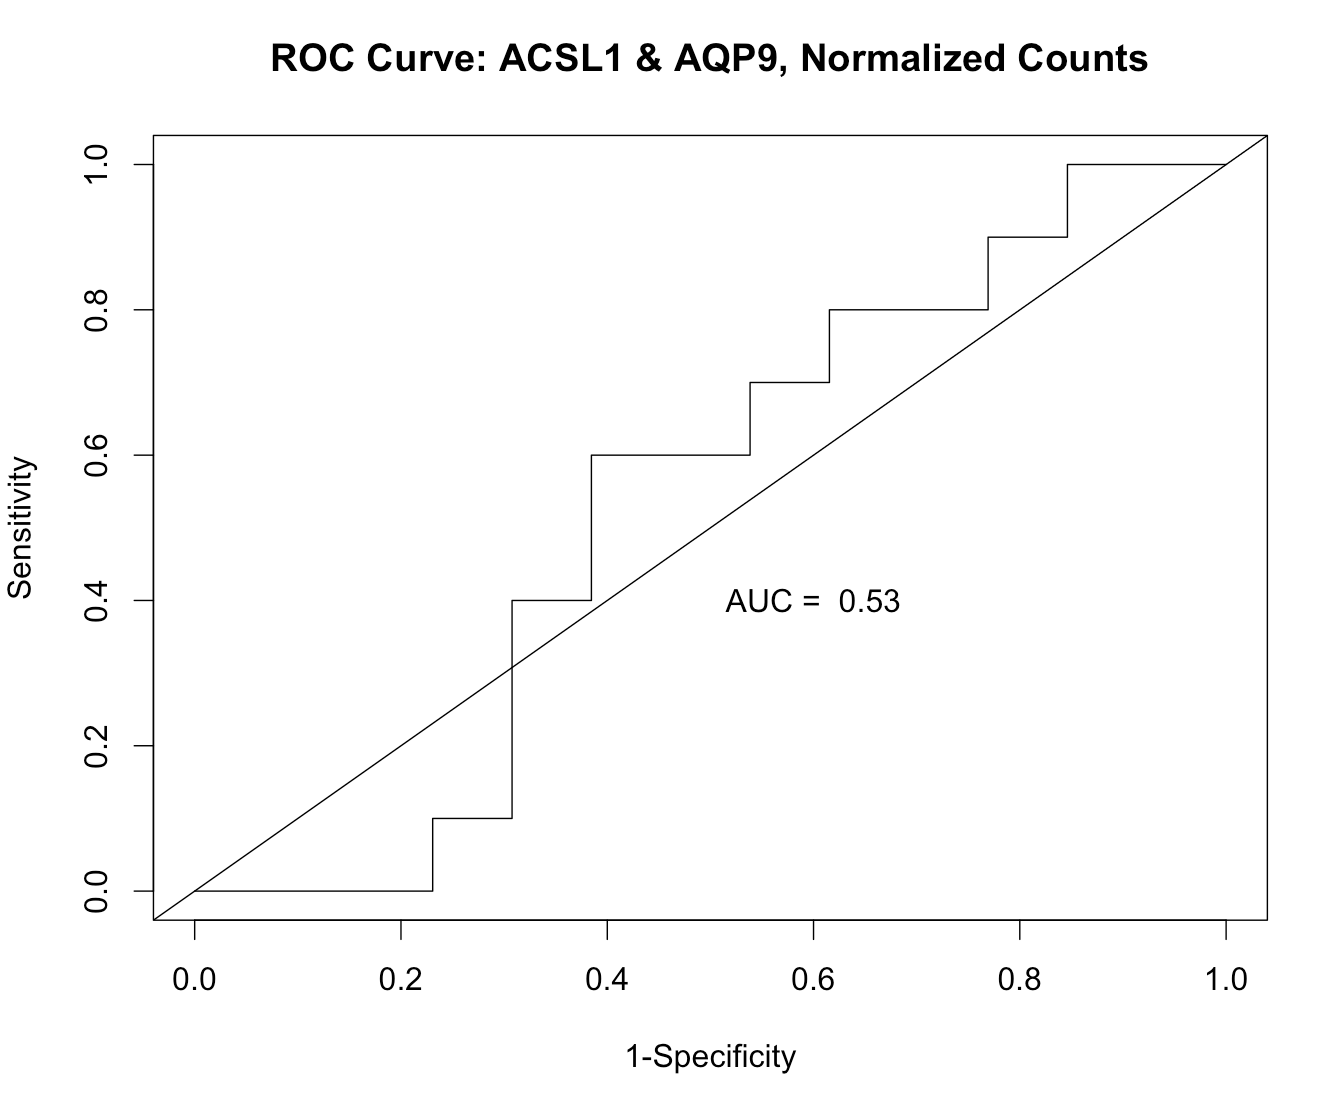
\includegraphics[scale=0.4]{../paper/figs/smoking3.png}
\end{frame}


\subsection{Pairwise Gene AUC Estimates}

\begin{frame}[fragile]
  	\frametitle{AUC Prediction Estimates for All PBMC Data Sets}
 		\begin{table}[h]
		\caption{AUC estimates for all exposures (via Super Learner \& cvAUC)} \label{tab:auc}
		\begin{center}
		\tabcolsep=0.11cm
		\scalebox{0.7}{
		\begin{tabular}{rlllllll}
  			\hline
 			& Benzene & Nickel & PAD & Smoking & Arsenic & Stress & Arthritis \\ 
 		 	\hline
			ACSL1 \& AQP9 & 0.9113095 & 0.75 & 0.5935673 & 0.5307692 & 0.1785714 & 				0.3397516 & 0.2944444 \\ 
  			NFKB1 \& IFNB1 & 0.939881 & 0.85 & 0.2251462 & 0.2653846 & 0.3285714 & 				0.3847826 & 0.437037 \\ 
  			PRG2 \& ACSL1 & 0.9204762 & 0.9 & 0.7339181 & 0.6615385 & 0.4666667 & 					0.3745342 & 0.3555556 \\ 
  			PRG2 \& CLEC5A & 0.9382143 & 1 & 0.5204678 & 0.6846154 & 0.5 & 0.3888199 & 			0.7148148 \\ 
  			NFKB1 \& CLEC5A & 0.9057143 & 0.8625 & 0.2704678 & 0.5769231 & 0.2428571 & 			0.2664596 & 0.6740741 \\ 
  			ACSL1 \& CLEC5A & 0.9150595 & 0.8375 & 0.6842105 & 0.6923077 & 0.15 & 					0.3409938 & 0.6703704 \\ 
   			\hline
		\end{tabular}
		}
		\end{center}
		\end{table} 
		\small AUC (of the ROC curve) provides the prediction accuracy given by the pairs of genes listed in the table above.
\end{frame}

\section{Conclusions}

\begin{frame}
        \frametitle{Contents}
        \tableofcontents[currentsection,currentsubsection,hideothersubsections,sectionstyle=show/shaded]
\end{frame}

\subsection{So What?}

\begin{frame}[fragile]
  	\frametitle{Why Should Anyone Care?}
 		\begin{itemize}
			\item The pair ACSL1 \& AQP9 looks promising because it predicts benzene exposure well, and a relatively low ability to predict nickel exposure. 
			\item This particular pair is completely ineffective in predicting other exposures in the PBMC data sets.
			\item Even a simple parametric method (LASSO) builds a relatively effective predictor of benzene exposure.
			\item Covariate removal via LASSO leaves AQP9 \& ACSL1 as the last two genes, which agrees with one of the six pairs. 
		\end{itemize}
\end{frame}

\subsection{Going Forward}

\begin{frame}[fragile]
  	\frametitle{Future Directions}
		\begin{itemize}
			\item Robustness of prediction to the choice of models in the Super Learner library warrants further investigation. 
			\item Gene Ontology.
		\end{itemize}
  		\begin{figure}
   			\href{https://github.com/nhejazi/PH240D-project2015}
         			{
\includegraphics[scale=0.25]{../paper/figs/octocat.png}}
			\caption{\url{https://github.com/nhejazi/PH240D-project2015}}
      		\end{figure}
\end{frame}

\begin{frame}[fragile]
  	\frametitle{Thank You!}
		\begin{itemize}
			\item {Alan Hubbard, Martyn Smith, \& the Superfund program} \\
			\item {\textit{Limma} (Bioconductor), Super Learner (Mark van der Laan), \& \textit{cvAUC} (Erin LeDell)} \\
			\item {All of you -- thanks for listening! You don't have to pay attention anymore...}
		\end{itemize}
\end{frame}



\end{document}
